\section{Chapter 2 - Mathematics Review}
\subsection{Thursday 01/16/2025}
\subsubsection{Chapter Math Outline}
The chapters over the next few lessons will include some math that will be used in different chapters.
\begin{itemize}
  \item Chapter 1: Linear algebra
  \subitem Matrices
  \subitem Eigenvalues
  \item Chapter 2: Convex Analysis
  \subitem Convexity
  \subitem Quadratic forms
  \subitem Taylor Series
\end{itemize}

\subsubsection{Linear Algebra Review}
A vector $\textbf{x} \in \mathbb{R}^n$ is defined as
\begin{align}
  \textbf{x} = 
  \begin{bmatrix}
     x_1 \\
     x_2 \\
     \vdots \\
     x_n
  \end{bmatrix}
\end{align}
This vector represents a direction and magnitude in $n$ dimensions. \\
The $l2$-norm of a vector is defned as
\begin{equation}
  \| \textbf{x} \|_2 = \sqrt{x_1^2 + x_2^2 + \dots x_n^2}
\end{equation}
Vector addition is defined as 
\begin{align}
  \textbf{x} + \textbf{y} = 
  \begin{bmatrix}
     x_1 \\ 
     x_2 \\ 
     \vdots \\
     x_n
  \end{bmatrix}
  + 
  \begin{bmatrix} 
    y_1 \\
    y_2 \\
    \vdots \\
    y_n
  \end{bmatrix}
   = 
   \begin{bmatrix} 
    x_1 + y_1 \\
    x_2 + y_2 \\
    \vdots \\
    x_n + y_n
  \end{bmatrix}
\end{align}
Scalar multiplication of a scalar $a \in \mathbb{R}$ with a vector $\textbf{x} \in \mathbb{R}^n$
\begin{align}
  a \textbf{x} = 
  \begin{bmatrix}
     a x_1 \\
     a x_2 \\
     \vdots \\
     a x_n 
  \end{bmatrix}
\end{align}
The dot product of two vectors $\textbf{x}, \textbf{y}, \in \mathbb{R}^n$ is defined as
\begin{align}
  \textbf{x}^\top \textbf{y} = 
  \begin{bmatrix}
     x_1 & x_2 & \dots & x_n
  \end{bmatrix}
  \begin{bmatrix}
    y_1 \\
     y_2 \\ 
     \vdots \\
     y_n
 \end{bmatrix}
\end{align}
With equivalent notation $\textbf{x}^\top \textbf{y} = \langle \textbf{x}, \textbf{y} \rangle$ \\
\begin{gather}
  \| \textbf{x} - \textbf{y} \|_2^2 = \| \textbf{x} \|_2^2 + \| \textbf{y} \|_2^2 - 2 \| \textbf{x} \|_2 \| \textbf{y} \|_2 \cos \theta \\
  \| \textbf{x} - \textbf{y} \|_2^2 = (\textbf{x} - \textbf{y})^\top (\textbf{x} - \textbf{y})
\end{gather}

The Cauchy-Schwarts Inequality is derived by the following
\begin{gather}
  \cos \theta = \frac{x^\top y}{\| x \| \| y \|} \\ 
  \frac{x^\top y}{\| x \| \| y \|} \leq 1 \\
  x^\top y \leq \| x \| \| y \|
\end{gather}

The triangle inequality is defined as
\begin{equation}
  \| \textbf{x} + \textbf{y} \| \leq \| \textbf{x} \| + \| \textbf{y} \|
\end{equation}

A matrix $A \in \mathbb{R}^{m \times n}$ is defined as 
\begin{align}
  A = 
  \begin{bmatrix}
     a_{11} & \dots & a_{1n} \\
    \vdots & \dots & \vdots \\
    a_{m1} & \dots & a_{mn}
  \end{bmatrix}
\end{align}
The transpose of a matrix $A^\top$ flips each value for the row and column  as such 
\begin{align}
  A^\top = 
  \begin{bmatrix}
     a_{11} & \dots & a_{1m} \\
    \vdots & \dots & \vdots \\
    a_{n1} & \dots & a_{nm}
  \end{bmatrix}
\end{align}
Matrix addition is element-wise and can be shown as such between two matrices $A,B \in \mathbb{R}^{m \times n}$
\begin{align}
  A + B = 
  \begin{bmatrix}
    a_{11} + b_{11} & \dots & a_{1n} + b_{1n} \\
    \vdots & \dots & \vdots \\
    a_{m1} + b_{m1} & \dots & a_{mn} + b_{mn}
  \end{bmatrix}
\end{align}
Scalar multiplication of a matrix $A$ with a scalar $\alpha$ is defined as 
\begin{align}
  \alpha A = 
  \begin{bmatrix}
     \alpha a_{11} & \dots & \alpha a_{1n} \\
    \vdots & \dots & \vdots \\
    \alpha a_{m1} & \dots & \alpha a_{mn}
  \end{bmatrix}
\end{align}
Matrix multiplication between two matrices $A \in \mathbb{R}^{m \times n}, B \in \mathbb{R}^{n \times p}$ is defined as 
\begin{align}
  AB = 
  \begin{bmatrix}
    a_{11} & \dots & a_{1n} \\
   \vdots & \dots & \vdots \\
   a_{m1} & \dots & a_{mn}
 \end{bmatrix}
 \begin{bmatrix}
  b_{11} & \dots & b_{1p} \\
 \vdots & \dots & \vdots \\
 b_{n1} & \dots & b_{np}
\end{bmatrix}
\end{align}
With the following properties
\begin{itemize}
  \item $AB \neq BA$
  \item $(ABC)^\top = C^\top B^\top A^\top $
\end{itemize}
The inverse of a matrix has the following properties
\begin{itemize}
  \item $AA^{-1} = I$
  \item $(AB)^{-1} - B^{-1} A^{-1}$
  \item $(B^\top)^{-1} = (B^{-1})^\top$
  \item $(A^{-1})^{-1} = A$
\end{itemize}
Orthonormal matrices have the properties
\begin{itemize}
  \item $O^\top O = I$
  \item $O^\top = O^{-1}$
\end{itemize}
Some following matrix partitions are useful
\begin{align}
  \begin{bmatrix}
     A_1 \\
     B_1
  \end{bmatrix}
  +
  \begin{bmatrix}
    A_2 \\
    B_2
 \end{bmatrix}
 =
 \begin{bmatrix}
  A_1 + A_1\\
  B_1 + B_2
\end{bmatrix}
\end{align}
\begin{align}
  \begin{bmatrix}
     A \\
     B
  \end{bmatrix}^\top
  = 
  \begin{bmatrix}
    A^\top & B^\top
 \end{bmatrix}
\end{align}
\begin{align}
  A
  \begin{bmatrix}
    B_1 \\
    B_2
  \end{bmatrix}^\top
  = 
  \begin{bmatrix}
    A B_1 & A B_2
 \end{bmatrix}
\end{align}

The determinant of a matrix $A \in \mathbb{R}^{n \times n}$ is calculated by subtracting the product of the diagonals of a matrix recursively. The minor of a matrix is the section of a matrix that is achieved when removing a section. Simply, the determinant of a matrix can also be defined as the product of the eigenvalues.
\begin{equation}
  \det A = \prod \lambda
\end{equation}

\subsubsection{Spaces}
A vector space is defined as a set of all vectors with some properties. We define a vector space $\mathbb{V}$
\begin{gather}
    u + v \in \mathbb{V} \\
    u + (v +w) = (u+v) + w \\
    u + v = v+ u 
\end{gather}
A linearly dependent system of vectors $v_i \in \mathbb{R}^n$ satifies the following for a set of scalars $c_i$
\begin{equation}
    c_1 v_1 + \dots + c_m v_m = 0
\end{equation}
The span of a set of vectors $v_i$ is the set of all vectors that can be created with a linear combination of those vectors.
\begin{equation}
    \{ x | c_1 v_1 + \dots + c_m  v_m = x  \}
\end{equation}
The basis of a space is the minimum number of vectors needed to span a vector space.

\subsection{Tuesday 01/21/2025}
\subsubsection{Matrix eigenvalues}
We define $\lambda$ as the eigenvalues of a matrix. We investigate what it means for matrices with different eigenvalues.
\begin{itemize}
  \item $\lambda_i \geq 0 \to $ Matrix $A$ is positive semi-definite
  \item $\lambda_i > 0 \to $ Matrix $A$ is positive definite
  \item $\lambda_i \leq 0 \to $ Matrix $A$ is negative semi-definite
  \item $\lambda_i < 0 \to $ Matrix $A$ is negative definite
  \item $\lambda_i < 0, \lambda_i > 0 \to $ Matrix $A$ is  indefinite
\end{itemize}

\subsubsection{Convex Sets}
A convex set is defined as a set where the line through all points is contained in the same set.
\\ \\
\textbf{Half Spaces}: 
\\
Half spaces are the space under a line, defined with the parameters $c \in \mathbb{R}^n z \in \mathbb{R}$,  
\begin{equation}
  \{ x | c^\top x \leq z, x \in \mathbb{R}^n \}
\end{equation}
A half space is open if the inequality is strict.

The intersection of a finite number of closed half spaces is known as a polytope. If a polytope is bounded on all sides, it is also known as a polyhedron.
\begin{figure}[h]
  \centering
  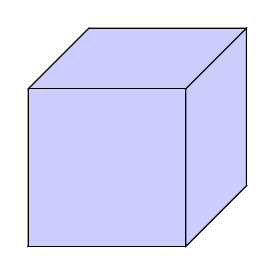
\begin{tikzpicture}
    \filldraw[fill=blue!20, draw=black] (0,0,0) -- (2,0,0) -- (2,2,0) -- (0,2,0) -- cycle;
    \filldraw[fill=blue!20, draw=black] (0,0,0) -- (2,0,0) -- (2,0,2) -- (0,0,2) -- cycle;
    \filldraw[fill=blue!20, draw=black] (0,0,0) -- (0,2,0) -- (0,2,2) -- (0,0,2) -- cycle;
    \filldraw[fill=blue!20, draw=black] (2,0,0) -- (2,2,0) -- (2,2,2) -- (2,0,2) -- cycle;
    \filldraw[fill=blue!20, draw=black] (0,2,0) -- (2,2,0) -- (2,2,2) -- (0,2,2) -- cycle;
    \filldraw[fill=blue!20, draw=black] (0,0,2) -- (2,0,2) -- (2,2,2) -- (0,2,2) -- cycle;
  \end{tikzpicture}
  \caption{A polyhedron}
  \label{fig:polyhedron}
\end{figure}
\\ \\ 
\textbf{Extreme Points}: 
\\
Consider a convex set $C \subseteq \mathbb{R}^n$. Let $z \in \mathbb{R}^n$, $z$ is an extreme point of $C$ if $z \in C$ and there are no $x,y \in C$ such that $z = (1-\lambda)x + \lambda y$. In other words, the point $z$ is not on a line defined by two points. The figure \ref{fig:2d_polyhedron} shows a polyhedron. It is impossible to represent the red points as a positive combination of two other points in this square. Therefore, they are extreme points.
\begin{figure}[h]
  \centering
  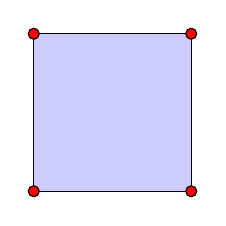
\begin{tikzpicture}
    \filldraw[fill=blue!20, draw=black] (0,0) -- (2,0) -- (2,2) -- (0,2) -- cycle;
    \foreach \x in {0,2} {
      \foreach \y in {0,2} {
        \filldraw[fill=red, draw=black] (\x,\y) circle (2pt);
      }
    }
  \end{tikzpicture}
  \caption{A 2D polyhedron with emphasized vertices}
  \label{fig:2d_polyhedron}
\end{figure}
\\ \\
\textbf{Convex combinations}: 
\\
Let $\textbf{x}_1, \textbf{x}_2, \dots, \textbf{x}_m$ be a set of $m$ vectors in $\mathbb{R}^n$. A convex combination of these vectors is a point of the form
\begin{gather}
  \lambda_1 \textbf{x}_1 + \dots + \lambda_m \textbf{x}_m
\end{gather}
where $\textbf{1}^\top \lambda = 1, \lambda \succeq 0$
\\ \\
\textbf{A Simplex}: 
\\
A simplex is the simplest possible polytope in a given dimension. Figure \ref{fig:simplexes} shows the simplexes in 0 to 3 dimensions.
\begin{figure}[h]
  \centering
  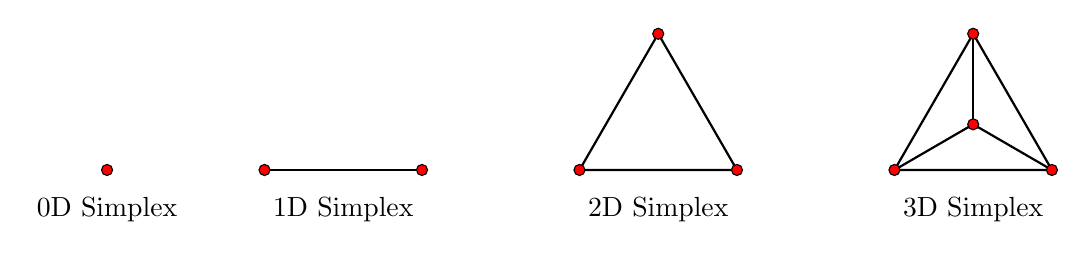
\begin{tikzpicture}
    % 0D simplex
    \filldraw[fill=red, draw=black] (0,0) circle (2pt);
    \node at (0,-0.5) {0D Simplex};

    % 1D simplex
    \draw[thick] (2,0) -- (4,0);
    \filldraw[fill=red, draw=black] (2,0) circle (2pt);
    \filldraw[fill=red, draw=black] (4,0) circle (2pt);
    \node at (3,-0.5) {1D Simplex};

    % 2D simplex
    \draw[thick] (6,0) -- (7,1.73) -- (8,0) -- cycle;
    \filldraw[fill=red, draw=black] (6,0) circle (2pt);
    \filldraw[fill=red, draw=black] (7,1.73) circle (2pt);
    \filldraw[fill=red, draw=black] (8,0) circle (2pt);
    \node at (7,-0.5) {2D Simplex};

    % 3D simplex
    \draw[thick] (10,0) -- (11,1.73) -- (12,0) -- cycle;
    \draw[thick] (10,0) -- (11,0.58) -- (12,0);
    \draw[thick] (11,1.73) -- (11,0.58);
    \filldraw[fill=red, draw=black] (10,0) circle (2pt);
    \filldraw[fill=red, draw=black] (11,1.73) circle (2pt);
    \filldraw[fill=red, draw=black] (12,0) circle (2pt);
    \filldraw[fill=red, draw=black] (11,0.58) circle (2pt);
    \node at (11,-0.5) {3D Simplex};
  \end{tikzpicture}
  \caption{Simplexes in 0D to 3D}
  \label{fig:simplexes}
\end{figure}
\\ \\
\textbf{Convex Hull}
\\ 
The convex hull of a set $S$ is defined as the smallest convex set that contains $S$. It is also defined as the intersection of all convex sets which contain $S$. Figure \ref{fig:nonconvex_convex_hull} shows the convex hull of a nonconvex set.
\begin{figure}[h]
  \centering
  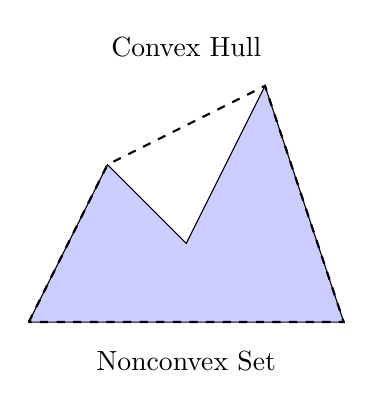
\begin{tikzpicture}
    % Nonconvex set
    \filldraw[fill=blue!20, draw=black] (0,0) -- (1,2) -- (2,1) -- (3,3) -- (4,0) -- cycle;
    \node at (2,-0.5) {Nonconvex Set};

    % Convex hull
    \draw[dashed, thick] (0,0) -- (1,2) -- (3,3) -- (4,0) -- cycle;
    \node at (2,3.5) {Convex Hull};
  \end{tikzpicture}
  \caption{A 2D nonconvex set and its convex hull}
  \label{fig:nonconvex_convex_hull}
\end{figure}
\\ \\ 
\textbf{Farkas Theorem}: 
\\
The Farkas Theorem is a theorem that allows for a certificate of feasibility (or infeasibility) of an optimization problem. With the variables $A \in \mathbb{R}^{m \times n}, b \in \mathbb{R}^n$, exactly one of the following two propositions is true.
\begin{itemize}
  \item $Ax = b, x \succeq 0$ for some $x \in \mathbb{R}^n$. In other words, $b$ is in the cone spanned by convex combinations of the columns of $A$.
  \item $A^\top y \succeq 0, b^\top y \leq 0$, for some $y \in \mathbb{R}^m$. In other words, the angle between $y$ and $b$ is greater than 90 and the angle between $y$ and every column of $A$ is less than 90. 
\end{itemize}

\begin{align}
  Ax = b \to 
  \begin{bmatrix}
     a_{11} x_1 + a_{12} x_2 + \dots a_{1n} x_n \\
     a_{21} x_1 + a_{22} x_2 + \dots a_{2n} x_n \\
     \vdots \\
     a_{m1} x_1 + a_{m2} x_2 + \dots a_{mn} x_n
  \end{bmatrix}
  =
  \begin{bmatrix}
    b_1 \\
    b_2 \\
    \vdots \\
    b_m
  \end{bmatrix}
\end{align}
\subsubsection{Convex Functions}
\textbf{Derivatives}: 
\\
Gradient refresher
\begin{align}
  \nabla f(x) = 
  \begin{bmatrix}
    \frac{d f}{d x_1} \\
    \frac{d f}{d x_2} \\ 
    \vdots \\
    \frac{d f}{d x_n}  
  \end{bmatrix}
\end{align}
A directional derivative is the transpose of the gradient times a direction $\nabla f(x)^\top d$. Consider a function $f : \mathbb{R}^n \to \mathbb{R}$ that is differentiable. A direction is a descent direction if $d^\top \nabla f(x) < 0$. The jacobian of a function is a generalized derivative for a function $f : \mathbb{R}^n \to \mathbb{R}^m$. It is defined as
\begin{align}
  J(x) = 
  \begin{bmatrix}
     \nabla f_1 (x)^\top \\
     \nabla f_2 (x)^\top \\
     \vdots \\
     \nabla f_m (x)^\top
  \end{bmatrix}
\end{align}
The hessian of a function is the second derivative of a function. The Hessian is symmetric as long as the mixed derivatives are equal to each other. 
\begin{align}
  H(f(x)) = 
  \begin{bmatrix}
     \frac{d^2 f}{d x_1^2} & \dots & \frac{d ^2 f}{d x_1 d x_n}   \\
     \vdots & \vdots & \vdots \\
     \frac{d^2 f}{d x_n d x_1} & \dots & \frac{d ^2 f}{d x_n^2}
  \end{bmatrix}
\end{align}
\\ \\
\textbf{Convex Functions}: 
\\
Let $C$ be a convex subset of $\mathbb{R}^n$, and f(x) be a real-valued function defined on $C$. The function $f$ is convex if Jensens inequality below holds. A function is strictly convex if the below property holds with strict inequality.
\begin{equation}
  f((1-\lambda)x_1 + \lambda x_2) \leq (1-\lambda) f(x_1) + \lambda f(x_2)
\end{equation}
In words, a function is convex if the line between any two points lies above every point of the function between those two points. Figure \ref{fig:convex_function} shows a convex function and how the line between any two points lies above the graph.
\begin{figure}[h]
  \centering
  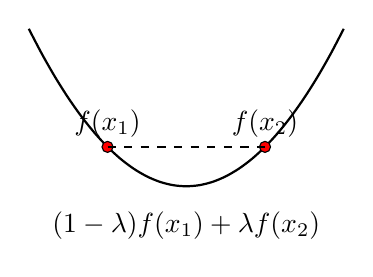
\begin{tikzpicture}
    % Convex function
    \draw[thick, domain=0:4, smooth, variable=\x] plot ({\x}, {0.5*\x*\x - 2*\x + 3});

    % Points on the function
    \filldraw[fill=red, draw=black] (1,1.5) circle (2pt) node[above] {$f(x_1)$};
    \filldraw[fill=red, draw=black] (3,1.5) circle (2pt) node[above] {$f(x_2)$};

    % Line between points
    \draw[dashed, thick] (1,1.5) -- (3,1.5);
    \node at (2,0.5) {$(1-\lambda)f(x_1) + \lambda f(x_2)$};
  \end{tikzpicture}
  \caption{A convex function and the line between two points}
  \label{fig:convex_function}
\end{figure}
Another way to define convex functions is with respect to the Hessian of the function $H(f(x))$. A function is convex if the Hessian of the function is positive semi definite $H(f(x)) \succeq 0$. Convexity can also be defined in sections of a function. For example, let $S$ be anon-empty open set in $\mathbb{R}^n$. If $f(x_0)$ is convex at the point $x_0$, then $H$ is positive semi-definite at that point.
\\ \\
\textbf{Example Problem}: 
\\
Determine if the following equation is convex
\begin{equation}
  f(x_1, x_2, x_3) = x_1^2 + x_2^2 + x_3^2 + 2x_1 x_2
\end{equation}
\begin{align}
  \nabla f(x) = 
  \begin{bmatrix}
     2 x_1 + 2x_2 \\
     2x_2 + 2x_1 \\
     2x_3
  \end{bmatrix}
\end{align}

\begin{align}
  \nabla^2 f(x) = 
  \begin{bmatrix}
     2 & 2 & 0 \\
     2 & 2 & 0 \\
     0 & 0 & 2
  \end{bmatrix}
\end{align}
Calculating the eigenvalues
\begin{align} \det
  \begin{bmatrix}
    2 - \lambda& 2 & 0 \\
    2 & 2 - \lambda & 0 \\
    0 & 0 & 2 - \lambda
  \end{bmatrix} 
\end{align}
\begin{gather}
  (2-\lambda)(2-\lambda)(2-\lambda) - 2(2)(2-\lambda) + 0= 0 \\
  (2-\lambda)^3 - 4(2-\lambda) = 0 \\
  (2-\lambda)((2-\lambda)^2 - 4) = 0 \\
  \lambda = [2, 0, 4]
\end{gather}
$\lambda = [0,2,4] \succeq 0$, therefore the hessian is positive semi-definite and the function is convex.
\subsubsection{Properties of Convex Functions}
\begin{itemize}
  \item if $f_i$ are convex, $\sum_i f_i(x)$ is convex
  \item if $f$ is convex, $\lambda f(x)$ is convex, where $\lambda is a scalar$
  \item Let $f$ be convex, and $g$ be an increasing function. The convex function $g(f(x))$ is also convex.
\end{itemize}

\subsubsection{Quadratic Forms}
The quadratic form of a vector $x \in \mathbb{R}^n$ with parameters $B in \mathbb{R}^{n \times n}, a \in \mathbb{R}^n, c \in \mathbb{R}$ is
\begin{equation}
  f(x) = \frac{1}{2} x^\top B x + a^\top x + c
\end{equation}

\subsection{Thursday 01/23/2025}
\subsubsection{Eigenvalues and Eigenvectors}
A non-singular matrix is a matrix $A$ that follows the property $\det A \neq 0 $.
\\ \\
\textbf{Eigenvalues}: 
\\ 
In order to calculate the eigenvalues of a matrix $A$, we solve the equation $\det (A - \lambda I) = 0$. For example, we take the matrix
\begin{align}
  A = 
  \begin{bmatrix}
     13 & -4 \\
     -4 & 7
  \end{bmatrix}
\end{align}
We subtract $\lambda$ from the diagonals to get 
\begin{align}
  A = 
  \begin{bmatrix}
     13 - \lambda & -4 \\
     -4 & 7 - \lambda
  \end{bmatrix}
  \\
  = (13-  \lambda)(7 - \lambda) - 16 = 0 \\
  \lambda_1 = 15, \lambda_2 = 5
\end{align}
Not all eigenvalues are always real. 
The number of eigenvalues is the same as the dimension of the matrix but is not always real.
\\ \\
\textbf{Eigenvectors}
\\
To find the eigenvectors $\nu$ of the matrix, we solve $(A - \lambda I )\nu = 0$.
\begin{align}
  A - \lambda I = 
(  \begin{bmatrix}
     13 & -4 \\
     -4 & 7
  \end{bmatrix}
  - 15
  \begin{bmatrix}
    1 & 0 \\
    0 & 1
  \end{bmatrix})
  \begin{bmatrix}
    v_1 \\
    v_2
  \end{bmatrix}
  =
  \begin{bmatrix}
    0 \\ 
    0
  \end{bmatrix}
  \\ 
  =
  \begin{bmatrix}
    -2 & -4 \\
    0 & 0
  \end{bmatrix}
  \begin{bmatrix}
    v_1 \\
    v_2
  \end{bmatrix}
  =
  \begin{bmatrix}
    0 \\ 
    0
  \end{bmatrix} \\
  -2 v_1 - 4v_2 = 0 \\
  v_1 + 2v_2 = 0 \\
  v_1 = - 2 v_2 \\
  \text{Infinite solutions, as long as the vector looks like }
  \begin{bmatrix}
    -2 a \\
    a
  \end{bmatrix}
\end{align}
Now we use the other eigenvalue $\lambda = 5$
\begin{align}
  A - \lambda I = 
(  \begin{bmatrix}
     13 & -4 \\
     -4 & 7
  \end{bmatrix}
  - 5
  \begin{bmatrix}
    1 & 0 \\
    0 & 1
  \end{bmatrix})
  \begin{bmatrix}
    w_1 \\
    w_2
  \end{bmatrix}
  =
  \begin{bmatrix}
    0 \\ 
    0
  \end{bmatrix}
  \\ 
  =
  \begin{bmatrix}
    8 & -4 \\
    -4 & 2
  \end{bmatrix}
  \begin{bmatrix}
    w_1 \\
    w_2
  \end{bmatrix}
  =
  \begin{bmatrix}
    0 \\ 
    0
  \end{bmatrix} \\
  \text{Infinite solutions, as long as the vector looks like }
  \begin{bmatrix}
    a/2 \\
    a
  \end{bmatrix}
\end{align}
\subsubsection{Convexity in Functions}
A bilinear function is a function in the form 
\begin{equation}
  f(x_1, x_2) = x_1 x_2
\end{equation}
The hessian of this function looks like
\begin{align}
  H = 
  \begin{bmatrix}
     0 & 1 \\
     1 & 0
  \end{bmatrix}
\end{align}
The eigenvalues of this matrix are $(-\lambda)^2 - 1 = 0, \lambda = \pm 1$.
This matrix is indefinite and therefore non-convex.
This function creates a saddle and is non-convex in both variables but is convex in either variable at a fixed falue of the other.